%%%%%%%%%%%%%%%%%%%%%%%%%%%%%%%%%%%%%%%%%%%%%%%%%%
\documentclass[b5paper,11pt, titlepage]{book}
%%%%%%%%%%%%%%%%%%%%%%%%%%%%%%%%%%%%%%%%%%%%%%%%%%
\usepackage[pdftex]{graphicx,color}
%\usepackage[T1,plmath]{polski}
\usepackage[cp1250]{inputenc}
\usepackage{indentfirst}
\usepackage[numbers,sort&compress]{natbib} % sort and compress citations
%\usepackage[none]{hyphenat} % brak podzia�?u wyraz??w
\usepackage{geometry}
\newgeometry{tmargin=3.6cm, bmargin=3.6cm, lmargin=3.2cm, rmargin=3.2cm}
\usepackage{multirow}
\usepackage{amsmath}
\usepackage{adjustbox} 

\renewcommand{\figurename}{Fig.}
\renewcommand{\tablename}{Tab.}

%%%%%%%%%%%%%%%%%%%%%%%%%%%%%%%%%%%%%%%%%%%%%%%%%%
\begin{document}
%%%%%%%%%%%%%%%%%%%%%%%%%%%%%%%%%%%%%%%%%%%%%%%%%%
%\title{\textbf{Modelowanie struktur anizotropowych \\Wst�pne badania eksperymentalne\\
%	\vspace{10cm}}
%\normalsize{Abstract} }
%\normalsize{W ramach projektu pt.: \\ \textit{Wp�yw jednoczesnego oddzia�ywania temperatury i wilgotno�ci \\na struktury anizotropowe: od teorii do bada� do�wiadczalnych\\}
%NCN OPUS 12}}
	
%{Micha� Jurek}

%\date{ }
	
%\date{Gda�sk, Maj 2018\\ (Nr Arch. 221/2018)}

%\maketitle
%\newpage
%\tableofcontents
%\newpage
%\listoffigures
%\listoftables
%\newpage

\chapter{Introduction to Structural Health Monitoring}
\textbf{Saeed Ullah}

\tableofcontents
\newpage
%%%%%%%%%%%%%%%%%%%%%%%%%%%%%%%%%%%%%%%%%%%%%%%%%%
\section{Structural Health Monitoring (SHM)}
%%%%%%%%%%%%%%%%%%%%%%%%%%%%%%%%%%%%%%%%%%%%%%%%%%
Numerous civil engineering and aerospace structures are exceeding or approaching their design lives. Therefore, assessing the condition of these structures is essential in order to determine their serviceability, safety
and load-carry capacity~\cite{Chang2000}. It is very crucial to monitor the health of structural elements in mechanical, civil, and aerospace industries where the presence of small defects may result in a very catastrophic failure. A defect or damage can be defined as any degradation in the structural parameters which changes the dynamic behavior of the structure~\cite{Chang2000}. These changes can be in a micro-scale level such as material matrix anomalies or in the macro-scale level such as cracks. Damage adversely affect the current or future performance of the system. Recently, damage detection methods have been widely studied for the purpose of locating and quantifying structural defects~\cite{Chang2000}. There are many ways and indicators for detecting damage in a structure such as variations in strain, natural frequencies, time signal, etc.~\cite{DeLuca2020}. Damage detection is usually accomplished in the context of one or more closely related disciplines which include: Structural Health Monitoring (SHM), Nondestructive Evaluation (NDE) also known as Nondestructive Testing (NDT), Condition Monitoring (CM), Health and Usage Monitoring System (HUMS), Damage Prognosis (DP) and Statistical Process Control (SPC)~\cite{Farrar2007, Farrar2012}. SHM can be defined as the process of implementing a damage detection and health assessment strategy for civil, mechanical engineering, or aerospace  infrastructure~\cite{Farrar2007, Farrar2012}. This process includes continuous monitoring of a mechanical system or structure using dynamic response measurements. For determining the current state of system health, the damage-sensitive features extracted from these measurements are used~\cite{Farrar2007, Farrar2012}. The output of these measurements can be periodically updated for long-term SHM. These measurements are very helpful in the case of an extreme event. SHM could be used for providing, in near real-time, reliable information and rapid condition assessment about the performance of the system~\cite{Farrar2012}. SHM aims to detect, identify, and characterize the damage and degradation in engineering structures. Sensors are used in the SHM system for monitoring physical quantities such as temperature, acceleration, humidity, tensile and compressive stress, and so on~\cite{Lamonaca2018}. SHM based techniques for damage detection needs few special characteristics such as (i) low possibility of missing the damage (ii) rapid calculation (iii) suitability for continuous on-line monitoring (iv) handling of huge information applicable for large engineering structures~\cite{lee2008overview}.

Tasks of SHM systems can be categorized as a process composed of four activities that form four important levels or elements, as shown in Fig. 1.1. These are: (i) damage detection, (ii) damage localization, (iii) damage size assessment, and (iv) life prognosis~\cite{stepinski2013advanced,TibaduizaBurgos2020,Scuro2018}. 
\begin{figure} [h!]
	\begin{center}
		\centering
		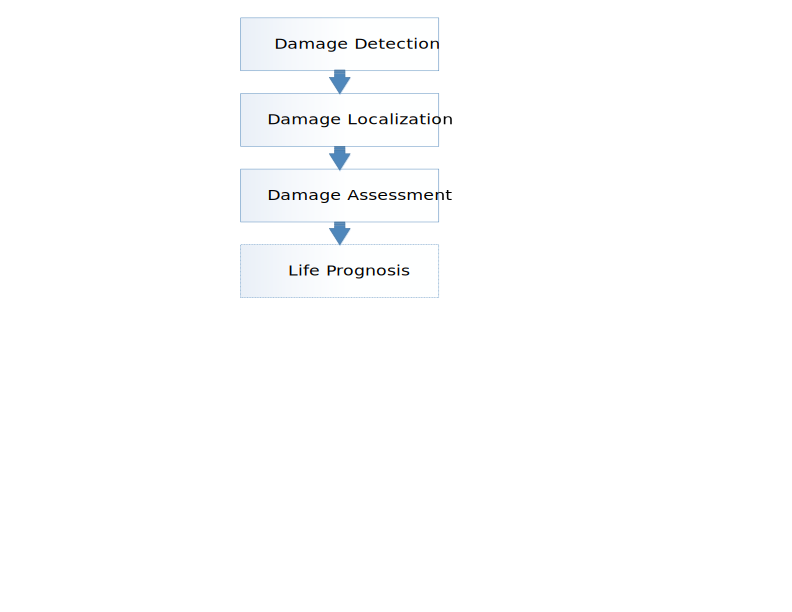
\includegraphics[width=0.5\textwidth]{fig1.1.png}
	\end{center}
	\caption{Main Levels of SHM Techniques} 
	\label{fig:fig1.1}
\end{figure}

According to these levels, detection gives a qualitative explanation that the damage may exist, localization gives an indication about the probable position of the damage, assessment indicates the estimation of damage severity by giving information about the size and type of damage and at last, the estimation of residual structural life is provided at prognosis stage. It also predicts possible failures or breakdowns. The first three levels (i.e. detection, localization, and assessment) are usually related to system identification, signal processing, and modelling aspects. The life prognosis level falls into statistical analysis, reliability, fatigue analysis, fracture mechanics, and design assessment fields. Many researchers have comprehensively investigated the prognosis level but currently, there are no commercially available solutions~\cite{stepinski2013advanced, TibaduizaBurgos2020}. 

\section{SHM and Nondestructive Testing/Evaluation (NDT/E)}
%%%%%%%%%%%%%%%%%%%%%%%%%%%%%%%%%%%%%%%%%%%%%%%%%%
Typically, SHM is identified as online�global damage identification method in structural systems. Whereas, NDT/E is usually performed as off-line in a local manner once the damage has been located or periodically, for improving the performance of a structure. However, it is not essential as NDT/E is also used as a monitoring tool for in situ structures such as rails and pressure vessels. NDT/E is primarily used for severity check and damage characterization when the damage location is already known~\cite{Farrar2007,Farrar2012}.

SHM involves integrating actuators and sensors, possibly smart materials, computational power, and data transmission within a structure in order to detect, assess, localize, and predict damage. A typical SHM system is concerned with online global damage identification in structures. SHM based systems are most often applied in civil engineering and aerospace. SHM systems employ NDT/E methods as tools, however, there are many differences in SHM and NDT/E operation principles~\cite{stepinski2013advanced}. 

NDT/E techniques are often bounded to single-point measurements. SHM methods allow for online monitoring of large structures and also can perform damage localization. With new sensors, SHM based methods are suitable for reliable continuous monitoring. For reliable damage detection, the SHM needs more state-of-the-art signal processing than classical NDT/E techniques~\cite{stepinski2013advanced}.

The main difference between SHM and NDT/E techniques can be observed from the hardware architecture. In the case of an SHM system, actuators and sensors are integrated with or built into the structure, while there is no integration involved with the structure in the case of NDT/E. NDT/E is an external system with an independent set of actuators and sensors~\cite{stepinski2013advanced}.
Most of the NDT/E techniques require component disassembly especially for those components that are inaccessible which results in interruption of the daily operation of the structural systems leading to downtime which consequently results in an increase in operational costs. In an effort to improve the integrity of structures, SHM technology has been introduced for the monitoring of civil, mechanical, and aerospace structures.  
NDT/E methods are often expensive, time-consuming, and labor-intensive, and they depend heavily on the skills and experience of the operator. NDT/E measurements are generally qualitative, there is no direct reliability of measurements to get verified. Proper experience and skilled judgment are required for NDT/E based techniques. Furthermore, safety precautions are also essential for most of the NDT/E methods. SHM is mainly
focused on condition-based maintenance. It is becoming more important nowadays
in various engineering fields such as mechanical, civil, and aerospace. NDT/E methods are basically localized in nature whereas SHM deals from a broader perspective. NDT/E requires prior knowledge of the location of damage whereas there is no such requirement in SHM. SHM is a better and modified version of NDT/E. SHM is able to save costs and maintain a proper level of safety taking into consideration the working conditions. SHM is used widely by the aerospace community, especially in a situation of aging of aircraft. NDT/E is slowly moving toward a more lasting attachment and continuous monitoring, and hence toward SHM. Smaller and cheaper sensors have been brought into the process of
changing from NDT/E to SHM.

\section{Advantages of SHM}
%%%%%%%%%%%%%%%%%%%%%%%%%%%%%%%%%%%%%%%%%%%%%%%%%%
Almost all government and private industries are interested in detecting damage in their products and manufacturing structures at the earliest feasible time. These industries carry out some form of SHM for such detection~\cite{Farrar2007}. The main aim of the SHM system is to maintain information on the state of the inspected structure for the purpose of finding structural defects before they reach critical levels. It also helps in providing adequate information for condition-based maintenance.

The SHM is an efficient approach for the regular monitoring of roads, bridges, skyscrapers, mechanical, civil, and aerospace structures. The new methods and technological developments are being employed in the SHM. The principal benefits of the employment of SHM include longer life spans, increased safety, detection of early risks, and cost-efficiency. Public safety is greatly improved with the use of new SHM methods. Regular monitoring and analysis assist in identifying design flaws. SHM is also helpful in recognizing environmental factors that may not have been taken into consideration during the construction process. Emergency maintenance and a continual preventative of different structures aids to improve their longevity. Another main advantage of SHM is that it greatly reduces short and long-term structural maintenance costs. Furthermore, structural integrity maintenance for a longer span of time lessens overall costs related to rebuilding and demolition~\cite{Lamonaca2018}. 

SHM offers an automated inspection process to reduce unessential maintenance tasks. Industries are using SHM as a tool for preventing sudden damage which yields essential benefits to the industries. SHM improves the safety and functionality of structures. SHM is useful in the timely warning of impending failures~\cite{TibaduizaBurgos2020}.

In an SHM system, data is gathered on realistic performance, which will help to design improved structures for the future. SHM is able to ensure safety and avoid the failure of the structure which in turn will save uncountable human losses due to accidents. In conventional systems, a considerable number of structures undergo regular assessment and maintenance for the purpose of ensuring the structural stability of the system. This number can easily be reduced by implementing an SHM system which will indicate the healthy structure to be unnecessary for the inspection.

\section{Different Types of SHM}
%%%%%%%%%%%%%%%%%%%%%%%%%%%%%%%%%%%%%%%%%%%%%%%%%%
Damage detection methods for SHM can be categorized into two main groups based on the type of information to be used: Local and Global methods. 

Local techniques monitor a tiny part of the structure surrounded by sensors using measurements of structural response. Acoustic emission, magnetic fields, radiography, eddy currents, ultrasonic waves, and thermal field are some examples which are commonly employed for local SHM~\cite{lee2008overview, stepinski2013advanced}.
\newline The global methods are executed when global motion is induced in the structure during its operation. Vibration-based methods are one of the examples of this class. Global methods are helpful when local damage has an influence on the behavior of the global structure in terms of space and time. 
As opposed to local methods, global methods have many benefits: 
\newline i) The whole structure can be measured with these methods by using a sparse sensor network.
\newline ii) It is not necessary to locate sensors near the damage.
\newline iii) Only a little information about the critical location is enough. 
Global methods also have some disadvantages: 
\newline i) The wavelength of vibrations is nearly equivalent to the dimension of the component or structure, therefore, these methods have relatively low sensitivity to small defects. 
\newline ii) Usually these methods are quite expensive.

Although the damage size and location are roughly estimated with these methods it can successfully be used for damage detection. The relationship between defects of structures and structural vibration is used in the health assessment. Global methods can be further divided into two types of methods: model-based and signal-based. The model-based methods utilize different kinds of models of a monitored structure to localize and detect the defect in the structure. These models use relations between particular defects and model parameters. In these methods, the comparison of damaged and undamaged structures are taken into account for detection and localization of damage. The relation between measured responses of the structures is employed in signal-based methods. Currently, signal features in time, frequency, and time/frequency domains are very popular. These methods are usually applied in diagnostics of reciprocating and rotating machinery for damage detection, but for damage assessment and localization additional information is also needed~\cite{stepinski2013advanced,Worden2007}. 

\section{Major Components of SHM}
%%%%%%%%%%%%%%%%%%%%%%%%%%%%%%%%%%%%%%%%%%%%%%%%%%
Mostly, an SHM system is represented as an online global damage identification system in structures. SHM systems are composed of three key elements: (i) A network of actuators and sensors, most likely smart materials, which are permanently attached to the structure. This aspect of SHM makes it different from conventional NDT/E techniques and it is mandatory for executing automated inspections. This step involves observation of the structure from arrays of sensors using regular sampled response measurements, storing the measured data, and transmitting data to the control center. (ii) On-board information handling and computing facilities. A large number of sensors are continuously producing a huge amount of data to be processed in real-time. Computational power and data transmission are employed within a structure for the purpose of detecting, localizing, assessing and predicting damage which can cause structure impairment now or in the future. (iii) Algorithms that analyze stored data from the structure with recently acquired data. Algorithms calculate a damage index and then inform about damage presence, localization, and type~\cite{stepinski2013advanced,Guemes2020a}.

For monitoring of possible changes in the structures, all SHM systems need a proper sensor network. The sensibility of the SHM system is usually associated with good interaction between the sensors and the structure. Therefore, it is very important to choose the appropriate sensors to be installed. During the implementation of a network of sensors in an SHM system, the information for obtaining defect identification, the material of the structure to inspect, the variables to sense or measure are considered. The next stage is data acquisition, also known as DAQ. In this stage, the signals produced by each sensor are obtained. At this stage, the characteristics of SHM systems, such as mobility, cost, scalability need to be considered. The information collected by the SHM system can be affected by sensor configuration, environmental and operational noise, or any other event. Many of these problems must be resolved before executing any analysis on the produced information for generalizing the techniques used for recognition, identification, or classification. This step is associated with preprocessing or signal conditioning. It can be performed with the use of hardware devices, software algorithms, or both. At last, data analysis tools are used for determining the existence of damage in the instrumented structure and for characterizing the possible source of the damage~\cite{TibaduizaBurgos2020,Crane2017}.
\section{Types of Sensors used in SHM}
%%%%%%%%%%%%%%%%%%%%%%%%%%%%%%%%%%%%%%%%%%%%%%%%%%
In the last few years, the structural engineering community is increasingly implementing sensor networks for SHM purposes of monitoring structures. For an SHM system, it is essential to acquire a proper assessment of a system dynamic response. There are several different types of sensors and data acquisition systems that can be applied to the SHM problem. The sensors employed in an SHM system are application-specific~\cite{Farrar2012}.

SHM sensing system consists of some or all of the following components:
\newline 1. Transducers that are responsible for converting changes in the field variable of interest i.e. temperature, strain, or acceleration to changes in an electrical signal i.e. resistance, voltage, or impedance.
\newline 2. Actuators that are responsible for applying a recommended input to the system i.e. a piezoelectric transducer attached to the surface of a structure.
\newline 3. Analogue-to-Digital (A/D) converters that are responsible for converting analogue electrical signal into a digital signal that can be processed on digital hardware. When an SHM system is using actuators, a Digital-to-Analogue (D/A) converter is also needed for converting a prescribed digital excitation signal to an analogue voltage which is useful for controlling the actuator~\cite{Farrar2012}. 

Damage detection for an SHM needs the employment of a set of sensors with the main function of capturing information which can be used for determining the state of the structure under inspection. Many SHM systems use the propagation of a signal that is produced by an actuator. The inspection also depends on the transducer type used for inspection and the type of propagating signals over the structure. The transducers employed in the SHM system should be light and small in size for the purpose of integration into the structure without any considerable impact on its behavior. With the increased implementation of SHM approaches, new sensors have been developed. These new sensors are very helpful in improving the ability of detection, characterization, and localization of defects in an SHM system. These advancements in sensors aim to reduce the weight and power consumption of the system. In addition, it also helps in resolving installation problems, and for improving operation facilities and subsequent data analysis. The following subsections illustrate some of the different types of sensors used in SHM systems. These sensors can be adapted for the inspection of both composite and metallic structures. Sensors can be categorized on the basis of physical variable which they sense or on the principle of transduction on which they are based. Some of these sensors, their advantages, disadvantages, and the inspected variable are shown in Tab 1.1~\cite{Farrar2012,TibaduizaBurgos2020}.

\subsection{Piezoelectric Sensors}
Piezoelectric materials are built from polymers and ceramic. Piezoelectric transducers (PZT) are a category of devices that satisfy most of the demands of SHM. PZT is lightweight, small in size, consumes a low amount of power, and is able to generate frequency response in a wider region. These transducers are less expensive and their size is relatively small in comparison to the size of the monitored structures. Some other advantages of piezoelectric sensors are: these sensors can be assembled in various shapes, such as longitudinal, rectangular, and circular. These transducers can be used for rapid and in situ SHM. PZT can easily be arranged as a network of sensors in order to record multipoint measurements on or under the surface of the monitored structure. However, the methods utilizing these transducers mostly needs a large number of data points and the baseline signal for the purpose of comparison with the damaged signal for authentic damage estimation~\cite{Farrar2012,Hameed2019}.
These transducers are mostly used for sensing and generation of guided waves. With PZT based transducers, it is easy to measure the vibration and acquire information about different variables, such as corrosion or deformation~\cite{TibaduizaBurgos2020,Mitra2016}. 

Arranging piezoelectric sensors for inspecting composite materials are represented as piezoelectric inspection. Piezoelectric inspection is considered as one of the active research areas of SHM based techniques. This technique uses a network of PZT transducers embedded into or attached to the host composite~\cite{Askaripour2019}.
\subsection{Fiber Optics}
Fiber optics are employed in those applications where high precision and electromagnetic-interference freedom is required. The principle underlying these sensors are based on white-light intervention, which can relate the complete shifting of a signal radiated from a light source with any physical variable. This type of sensors is useful for measuring temperature, acceleration, vibrations, pressure, rotation, deformation, material concentrations, and shifting. For deformation measurements, Fiber Optics Sensors (FOS) and Fiber Bragg Grating (FBG) sensors are mostly used. FOS are less costly, usually contain multimode fibers and auto-compensate for temperature changes. Whereas, FBG sensors are used as selective filters of any wavelength~\cite{TibaduizaBurgos2020}. 
\subsection{Microelectromechanical Systems (MEMS)}
Miniaturization techniques are used in the construction of this type of sensors and it combines different types of transducers. These sensors are very beneficial in case of the costs of maintenance and implementation. MEMS sensors have some other attractive features too, such as their small size or their ability of easy connectivity with a wireless sensor network. It is even possible to find sensors that use inductive, capacitive, optical effects, or piezoelectric. In addition, actuators can also be included. Generally, MEMS are composed of the integration of various types of sensors. MEMS are used for measuring the magnitude of diverse variables, such as angular velocity (gyroscopes), displacement, acceleration, and deformation. This type of sensor provides high sensitivity, the integration of communication systems, responses at low frequencies, and the measurement of multiple variables. Recently, the use of MEMS sensors has significantly increased due to the mentioned factors~\cite{Farrar2012, TibaduizaBurgos2020}.

\begin{table}[h]
	\centering
	\caption{Details of Various Types of Sensors Used in SHM}
	\begin{adjustbox}{width=\textwidth-0.01pt,center}
\begin{tabular}{ccccc}
	\hline
	\textbf{Sensor Type}                                                                                                 & \textbf{Technology}          & \textbf{Variable to Measure}               & \textbf{Advantages}                                                                  & \textbf{Disadvantages}                                            \\ \hline
	\multirow{5}{*}{Piezoelectric}                                                                                       & PZT                          & Acceleration                               & Low Cost                                                                             & Thermal Sensitivity                                               \\ \cline{2-5} 
	& PVDF                         & Deformation                                & Low Price                                                                            & Aging                                                             \\ \cline{2-5} 
	& \multirow{3}{*}{P(VDF-TrFE)} & Corrosion                                  & Integration Possibilities                                                            &                                                                   \\ \cline{3-5} 
	&                              & Vibration                                  & \multicolumn{1}{l}{}                                                                 & \multicolumn{1}{l}{}                                              \\ \cline{3-5} 
	&                              & Displacement                               & \multicolumn{1}{l}{}                                                                 & \multicolumn{1}{l}{}                                              \\ \hline
	\multirow{6}{*}{Fiber Optics}                                                                                        & \multirow{5}{*}{FOS}         & Rotation                                   & \begin{tabular}[c]{@{}c@{}}Electromagnetic Interference\\  Immunity\end{tabular}     &                                                                   \\ \cline{3-5} 
	&                              & Acceleration                               &                                                                                      & Fragility                                                         \\ \cline{3-5} 
	&                              & Vibrations                                 & Integration Possibilities                                                            & \multicolumn{1}{l}{}                                              \\ \cline{3-5} 
	&                              & Pressure                                   & \multicolumn{1}{l}{}                                                                 & \multicolumn{1}{l}{}                                              \\ \cline{3-5} 
	&                              & Shifting                                   & \multicolumn{1}{l}{}                                                                 & \multicolumn{1}{l}{}                                              \\ \cline{2-5} 
	& FBG                          & Deformation                                & High precision                                                                       & High price                                                        \\ \hline
	\multicolumn{1}{l}{\multirow{5}{*}{\begin{tabular}[c]{@{}l@{}}Microelectromechanical\\ Systems (MEMS)\end{tabular}}} & MEMS                         & Deformation                                & Low cost                                                                             & \begin{tabular}[c]{@{}c@{}}High-frequency\\ Response\end{tabular} \\ \cline{2-5} 
	\multicolumn{1}{l}{}                                                                                                 & \multirow{4}{*}{NEMS}        & Deformation                                & \begin{tabular}[c]{@{}c@{}}Different Kinds of\\ Sensors and\\ Variables\end{tabular} & \multicolumn{1}{l}{}                                              \\ \cline{3-5} 
	\multicolumn{1}{l}{}                                                                                                 &                              & Displacement                               & Wireless Connection                                                                  & \multicolumn{1}{l}{}                                              \\ \cline{3-5} 
	\multicolumn{1}{l}{}                                                                                                 &                              & \multicolumn{1}{l}{Acceleration Gyrometer} & Small Size                                                                           & Fragility                                                         \\ \cline{3-5} 
	\multicolumn{1}{l}{}                                                                                                 &                              & Shifting                                   & \multicolumn{1}{l}{}                                                                 & \multicolumn{1}{l}{}                                              \\ \hline
\end{tabular}
\end{adjustbox}
\end{table}
\section{Guided Waves Based SHM}
%%%%%%%%%%%%%%%%%%%%%%%%%%%%%%%%%%%%%%%%%%%%%%%%%%
\subsection{Guided Waves}

Recently, three types of SHM techniques have been successively developed: (1)  SHM based on vibrations~\cite{MMaia}; (2) Electromechanical Impedance (EMI) based SHM~\cite{Fiborek2018}; and (3) Guided wave-based SHM~\cite{Mei2019,Tian2015,Park2014,Sikdar2019,Girolamo2018,Rogge2013,Kudela2018}. Vibration-based SHM techniques detect damage by measuring vibration signals on structures. These techniques identify local defects by detecting changes in modal shapes, natural frequencies, or dynamic responses. EMI based techniques identify changes in structures by measuring the EMI of a PZT transducer, which is connected to (or embedded into) the monitored structure. Guided Waves (GWs) are elastic waves that are propagating along a path determined by the structure boundaries. GWs are of huge concern for NDT/E and SHM of engineering structures such as rails, aircraft components, and oil and gas pipelines. Developing a GWs based technique needs attentive understanding obtained over-analysis and modelling of mode-damage interaction and wave propagation due to the dispersion and multimodal character of GWs~\cite{Lugovtsova2019}. These techniques have several advantages: (1) A relatively small wavelength provide plentiful interaction of the GWs and minor damage; (2) The excitation frequency of these waves is very high, therefore, signals of the ambient frequencies are barely distracted; (3) These waves can travel relatively long distances within the structure under investigation; (4) It provides better sensitivity to a variety of defects or damage types and the extent of the monitored area.

Velocity, scattering, attenuation, and mode conversion are some of the features which are used for indicating changes in structural dynamics~\cite{Wang2020,Mitra2016}. In these techniques, an actuator is used which travels through the structure for generating the waves. Signals are received by the transducers at one or multiple locations which are then analyzed for the identification of defect or damage. In GWs, damage can be detected and monitored with a very small number of transducers~\cite{Munian2018}. In many GWs based SHM techniques, groups of actuators/sensor are adjusted on a plate which not only identifies the existence of damage but also locate the damage~\cite{Farrar2012}.

In the GWs based SHM system, usually, an array of PZTs is used for sensing and excitation of signals. It provides the ability of online monitoring and the permanent integration of modifications in GWs propagation. However, the problem of applying an array consisting of few PZTs for damage localization is that the resolution of the damage imaging can be very low. Whereas, the application of a very dense array of PZTs is also not feasible. This problem can be solved by using Scanning Laser Doppler Vibrometry (SLDV). SLDV is capable of measuring GWs in a very dense grid of points over the surface of a large specimen. This collection of signals is known as full wavefield~\cite{Wandowski2011,Radzienski2019}.

\subsection{Lamb Waves}

Lamb wave is a form of ultrasonic guided waves which propagates in plate-like structures ~\cite{Lamb1917}. Lamb waves interrogation of structures is an appealing SHM technique for damage detection and monitoring. Lamb waves have the ability to travel longer distances with minimum dispersion. These waves are also highly sensitive towards detecting small defects. Damage in structures using Lamb waves can be evaluated by analyzing modifications in the propagation of Lamb waves considering backward and forward scattering~\cite{Hameed2019b}. These waves provide more information about the presence, size, type, location, and severity of damage than frequency response techniques~\cite{Kessler2002}. Both internal and external defects in large monitoring structures can be inspected with Lamb waves. Due to these reasons, Lamb waves have been proved to be very suitable for the detection of damage in plate-like structures~\cite{Kudela2018a}. For the generation and detection of Lamb waves, the Lead Zirconate Titanate (PZT) are mostly used~\cite{Journal}. Both contact and non-contact type transducers can be used for the generation of Lamb waves. Sophisticated signal-processing techniques are used for the processing of the dynamic response signal received by PZT transducers. Damage information can easily and accurately be extracted with efficient signal-processing techniques~\cite{Hameed2019a,Su2004}. 

Lamb waves are guided by the free surfaces of plates. The order of wavelengths and magnitude of these waves is the same as the thickness of the plate. Lamb waves couple shear and longitudinal waves within a plate. In order to use lamb waves for SHM, it is beneficial to have a waveform that is efficiently recognizable before and after propagation through the plate. The frequency dependency of wave speed in Lamb waves makes these waves dispersive. However, different frequency components are propagated at different velocities within the plate. A narrow-band frequency is preferred for maximizing the effectiveness of Lamb waves. By using driving frequency various Lamb wave modes are initially well-spaced and hence the modes of interest are comparatively nondispersive~\cite{Kessler2002}. By choosing a suitable driving frequency, the response of the input signal is recorded at receiving sensors with extremely minimal interference~\cite{Farrar2012} 

The propagation of Lamb waves can be categorized into either Symmetric ($S_0$) or Antisymmetric ($A_0$) modes. $A_0$ mode of waves can travel longer distances with little dispersion~\cite{Kessler2002}. The $A_0$ mode of Lamb waves is very useful for damage identification. The wavelength and wave velocity of $A_0$ is relatively smaller. The smaller wavelength of $A_0$ mode is very helpful because for interacting with the damage, the half wavelength of a selected wave mode must be smaller or equal to the damage size. $A_0$ modes can also be easily generated by surface mounted transducers~\cite{Ricci2016}. Usually $A_0$ mode of Lamb waves is preferred over $S_0$ mode because $S_0$ mode is very faster which results in arrival time measurement complexity~\cite{Askaripour2019}.   

The main problem of Lamb waves is that it is an active technique. It needs a regular supply of function generating signal and voltage. The resulting data of Lamb waves is also more complicated than many other techniques. Therefore, the interpretation of these signals is also very difficult~\cite{Kessler2002}.

Despite an extensive number of research efforts, Lamb waves based real engineering applications are still limited. This is mainly because of the complexity of the propagation of Lamb waves, i.e. dispersion, multimodal nature, possible reflections from boundaries and also more structural features which generate a wave field which is laborious to analyse~\cite{stepinski2013advanced}.

\subsection{Scanning Laser Doppler Vibrometer (SLDV):}
Laser Doppler Vibrometer (LDV) works on the principle of the Doppler shift.  LDV is highly applicable for the measurement of the out-of-plane surface velocities. LDV measures these velocities with high accuracy and in non-contact mode during guided wave propagation~\cite{Mitra2016}. LDV sensing system has been widely used for sensing of guided wave and more particularly for Lamb waves~\cite{Mitra2016}. 

Generally, an LDV sensing system contains a laser head that launches a laser beam and then records the reflected beam of the vibrating surface. A demodulator is used for transforming the information of the reflected beam into velocity measurements, and a controller is used to deflect the optical mirrors for the purpose of proper alignment of the laser beam. A simpler version of the LDV sensing system is a single point that can perform only a single point measurement. The Scanning LDV (SLDV) is capable of recording and measuring the vibrations at various points on a predefined grid. SLDV facilitates high resolution, rapid, and precise imaging of the wave response of a structure in a non-contact way~\cite{Mitra2016}. SLDV enables measurement of full wavefield of a structure instead of single point measurements usually acquired by conventional sensors. SLDV is useful for measuring the velocity of the inspected area in points associated with a predefined grid. SLDV based measurements can be combined with adequate imaging and signal processing algorithms for the purpose of damage identification. High resolution based SLVD measurements provides very detailed visualization of multiple damage of different types~\cite{Kudela2015}.

A layout of mirrors is equipped with SLDV which is helpful for changing the angle of measurement beams. A digital camera is also equipped with SLDV which is helping for defining a measurement grid precisely on the selected area of the object of interest. Furthermore, a screen of monitor is used for the visualization of the grid. 3D vibrometers are used for providing information of the monitored object in three dimensions which is very helpful in many cases. However, acquiring 3D measurements are more difficult than 1D measurements because 3D measurements need an added alignment of the three laser heads~\cite{Ostachowicz2014}.

Recently, notable progress has been carried out in the measurement techniques such as shearographic interferometry and SLDV. These techniques allow analysis of a full wavefield of elastic waves. The advancement in these techniques initiated new opportunities for the various types of damage detection problems in structures~\cite{Mitra2016}.

Some of the disadvantages of SLDV are: (1) The inspected object surface has to be characterised by proper reflectivity. In other case, the acquired signal-to-noise ratio is low. (2) For a specified time, the measurements can only be performed at one point in space. (3) SLDV is very expensive. (4) The measurements need to be repeated many times for full field Lamb wave registration at a dense grid of points~\cite{Ostachowicz2014}.
(5) High resolution measurement of SLDV takes much time and needs a large amount of hard drive space.

\section{SHM in Composite Structures}
%%%%%%%%%%%%%%%%%%%%%%%%%%%%%%%%%%%%%%%%%%%%%%%%%%
In recent years, various industries are progressively employing composite structures for achieving the desired performance in a wide area of applications~\cite{Hameed2019b}. The use of composite structures is growing rapidly due to its simple structure, high specific strength, lightweight, and many other desired mechanical properties~\cite{Radzienski2019}. 

Maintenance is required for the composite materials because of less frequent and complex material failures in them. The failure measurement in composite structures depends upon many quantitative and qualitative factors such as structural stiffness of the composite, the strength of the structures, resistance to corrosion, resistance to impact, fatigue due to loading and unloading cycles, resistance toward lightning and thunderstorms, and yield capacity of the composite~\cite{Rahul2018}. Different forms of damage can occur in composite materials such as debonding, matrix cracking, fiber breakage, and delamination~\cite{Yu2019,Fakih2019}. Composites structures are very sensitive to impact loads. Even a low-intensity and the low-velocity impact can commence matrix cracks in composites. The matrix cracks in composites then lead to delamination which is one of the most common susceptible defects in composites structure. Delamination can grow and badly affect the structural integrity and mechanical properties of the composites~\cite{Munian2018}. 

In recent decades, many researchers have developed numerous intelligent and computational based SHM techniques for composites structures. Eddy currents (electromagnetic testing), acoustic emissions, optical methods, ultrasonic inspection, vibration analysis, thermography, radiography, and Lamb waves are extensively used damage detecting techniques in composite structures~\cite{Rahul2018}. Guided Lamb waves are broadly recognized as one of the most promising tools for significant identification of defects in composite structures~\cite{stepinski2013advanced,Ricci2016}. Guided wave-based SHM technologies have been widely applied for detecting various types of damages in composite structures, including debonding ~\cite{Sikdar2019}, delamination ~\cite{Tian2015,Park2014},  and impact damage ~\cite{Girolamo2018,Rogge2013,Kudela2018}. Lamb waves based SHM techniques are commonly used for damage detection in composite materials. 

Lamb waves based damage detection, identification, and localization of damage for composite structures have extensively been studied in the literature. Yang et al. ~\cite{Yang2019} evaluated the size, location, and shape of damage with Lamb waves by using PZT wafer transducers in composite materials. Hameed et al. ~\cite{Hameed2019b} developed an efficient damage detection technique by introducing quantitative size estimation and transverse damage localization for composite materials with the use of Lamb waves. Li et al. ~\cite{Li2012} developed a technique based on the second harmonic Lamb waves propagation for assessing the thermal fatigue damage in composite structures. Zak et al. ~\cite{Zak2012} used laser scanning vibrometry for experimental measurements for damage detection in metal and thin-walled composite structures with the use of guided Lamb waves. They applied the spectral finite element method for numerical investigations. Fakih et al. ~\cite{Fakih2019} developed a Lamb wave-based technique for the detection, localization, and assessment of the severity for barely visible indentation damage in composite structures. Toyama and Takatsubo ~\cite{Toyama2004} used an Acoustic Emission (AE) transducer and Angle Beam Transducer (ABT) for the detection of impact damage in composite laminates using $S_0$ mode of Lamb waves. Rauter et al. ~\cite{Rauter2015} developed an impact damage detection method for composite structures based on nonlinear Lamb waves.

\section{Major Challenges in SHM}
%%%%%%%%%%%%%%%%%%%%%%%%%%%%%%%%%%%%%%%%%%%%%%%%%%
Although SHM has numerous advantages, like it increases the life span, maintaining only when needed, and it improves public safety. However, there are certain limitations to SHM. SHM systems can be unreliable, expensive, and very complicated for an industrial manager to understand. It is very difficult to convince the industrial managers and structural system owners that the SHM is more beneficial than their current maintenance system. The variations in structures also need unique monitoring techniques to be employed with each structure which is an enormous task and also prone to defects. One main challenge is the lack of available data from damaged systems that are needed in many situations. Another problem is making repeatable and accurate measurements for a longer time on complex structures generally operating in adverse environments. Another significant challenge is the development of the capability of defining the properties of the required sensing system before field deployment. Some other challenges of SHM are power sources, sensor failures, failures of signal processing methods, data collection and transferral~\cite{Farrar2007}.

\section{Conclusion}
%%%%%%%%%%%%%%%%%%%%%%%%%%%%%%%%%%%%%%%%%%%%%%%%%%
In this chapter, damage, types of damage, SHM, the need for carrying out SHM in various industries, and the main levels of SHM along with the functionalities of every level are elaborated. Firstly, the damage is detected next the location of the damage is identified after that the size and type of damage are estimated and in the end, the remaining life of the structure is evaluated. The interrelation and major differences between SHM and NDT/E techniques are also demonstrated. Furthermore, the intentions and benefits of carrying out SHM are presented. Different kinds of SHM based techniques and the basic components of SHM based techniques are described. Various types of sensors used for implementing SHM techniques are explained. PZT based transducers are usually preferred over fiber optics and MEMS sensors due to its smaller size and low cost. Moreover, guided waves, Lamb waves, and SLDV are presented. The use of guided waves, Lamb waves, and SLDV in SHM are also explained. Guided Lamb waves are usually preferred over vibrations and EMI for implementing SHM techniques due to its longer propagation distances and suitability for distinguishing smaller defects. Furthermore, various types of guided waves based damage detection, localization, and assessment techniques implemented in composite materials are described. In the end, major challenges of SHM are discussed because implementing SHM techniques may encounter some problems such as lack of available data, sensor failures, high cost, and accuracy of damage identification in real-world scenarios.
%%%%%%%%%%%%%%%%%%%%%%%%%%%%%%%%%%%%%%%%%%%%%%%%%%
%\subsection{Description}
%%%%%%%%%%%%%%%%%%%%%%%%%%%%%%%%%%%%%%%%%%%%%%%%%%
%text
%%%%%%%%%%%%%%%%%%%%%%%%%%%%%%%%%%%%%%%%%%%%%%%%%%

%\begin{figure} [h!]
%	\begin{center}
		%\includegraphics[width=14cm]{Graphics/bc.jpg}
%	\end{center}
%	\caption{Figure caption.} 
%	\label{fig:bc}
%\end{figure}

%%%%%%%%%%%%%%%%%%%%%%%%%%%%%%%%%%%%%%%%%%%%%%%%%%

%\begin{table}[h]
%\centering
%	\caption{Table caption}
%	\begin{tabular}{cccc}
%		\hline
%	\textbf{a}	& \textbf{x} & \textbf{y} & \textbf{z} \\
%		\hline
%		-50 & -0.289 & -0.289 & -0.598\\ 
%		-40 & -0.248 & -0.248 & -0.512\\ 
%		\hline 
%	\end{tabular} 
%	\label{tab:xyz}
%\end{table}
%%%%%%%%%%%%%%%%%%%%%%%%%%%%%%%%%%%%%%%%%%%%%%%%%%

%The scheme of experimental setup is shown in Fig.~\ref{fig:bc}.  
%The values are collected in Tab.~\ref{tab:xyz}.


%The details are described in a book~~\cite{udd2011fiber}. 

%Similar case was analysed~\cite{Badrinarayanan2017a} by Hill et al.
%Additional information:
%\begin{itemize}
%\item fonts Times New Roman, 11pt
%\item keep figures separately in greyscale with resolution 600 dpi (publisher requirement)
%\item 20-30 pages
%\item Bibliography~\cite references in the order of citations within the text
%\end{itemize}

\bibliography{report} % 
%bibliography data in report.bib
\bibliographystyle{abbrv}
% makes bibtex use spiebib.bst


%%%%%%%%%%%%%%%%%%%%%%%%%%%%%%%%%%%%%%%%%%%%%%%%%%
\end{document}
%%%%%%%%%%%%%%%%%%%%%%%%%%%%%%%%%%%%%%%%%%%%%%%%%%
